\documentclass[a4paper]{article}
\usepackage{student}

% Metadata
\date{\today}
\setmodule{CS110: Computer Architecture}
\setterm{Spring, 2024}

%-------------------------------%
% Other details
% TODO: Fill these
%-------------------------------%
\title{Assignment 4: Digital circuit}
\setmembername{He Yaoyu}  % Fill student name
\setmemberuid{2022533089}  % Fill  student id

%-------------------------------%
% Add / Delete commands and packages
% TODO: Add / Delete here as you need
%-------------------------------%
\usepackage{amsmath,amssymb,bm}
\usepackage{tikz}
\usetikzlibrary{automata, positioning, arrows}
\usepackage{hyperref}

\newcommand{\KL}{\mathrm{KL}}
\newcommand{\R}{\mathbb{R}}
\newcommand{\E}{\mathbb{E}}
\newcommand{\T}{\top}

\newcommand{\expdist}[2]{%
        \normalfont{\textsc{Exp}}(#1, #2)%
    }
\newcommand{\expparam}{\bm \lambda}
\newcommand{\Expparam}{\bm \Lambda}
\newcommand{\natparam}{\bm \eta}
\newcommand{\Natparam}{\bm H}
\newcommand{\sufstat}{\bm u}

% Main document
\begin{document}
    % Add header
    \header{}
\textcolor{red}{\textbf{Attention: }}
\textbf{Recommend using \LaTeX to complete your work. You can use any tool, such as Logisim, Visio, Draw.io, PowerPoint, etc., to create diagrams. However, handwritten or hand-drawn content is not acceptable.}

\section{Combinational logic}
Analyze the circuit shown in Fig.~\ref{fig:circuit} and answer the following questions:
\begin{figure}[htbp]
    \centering
    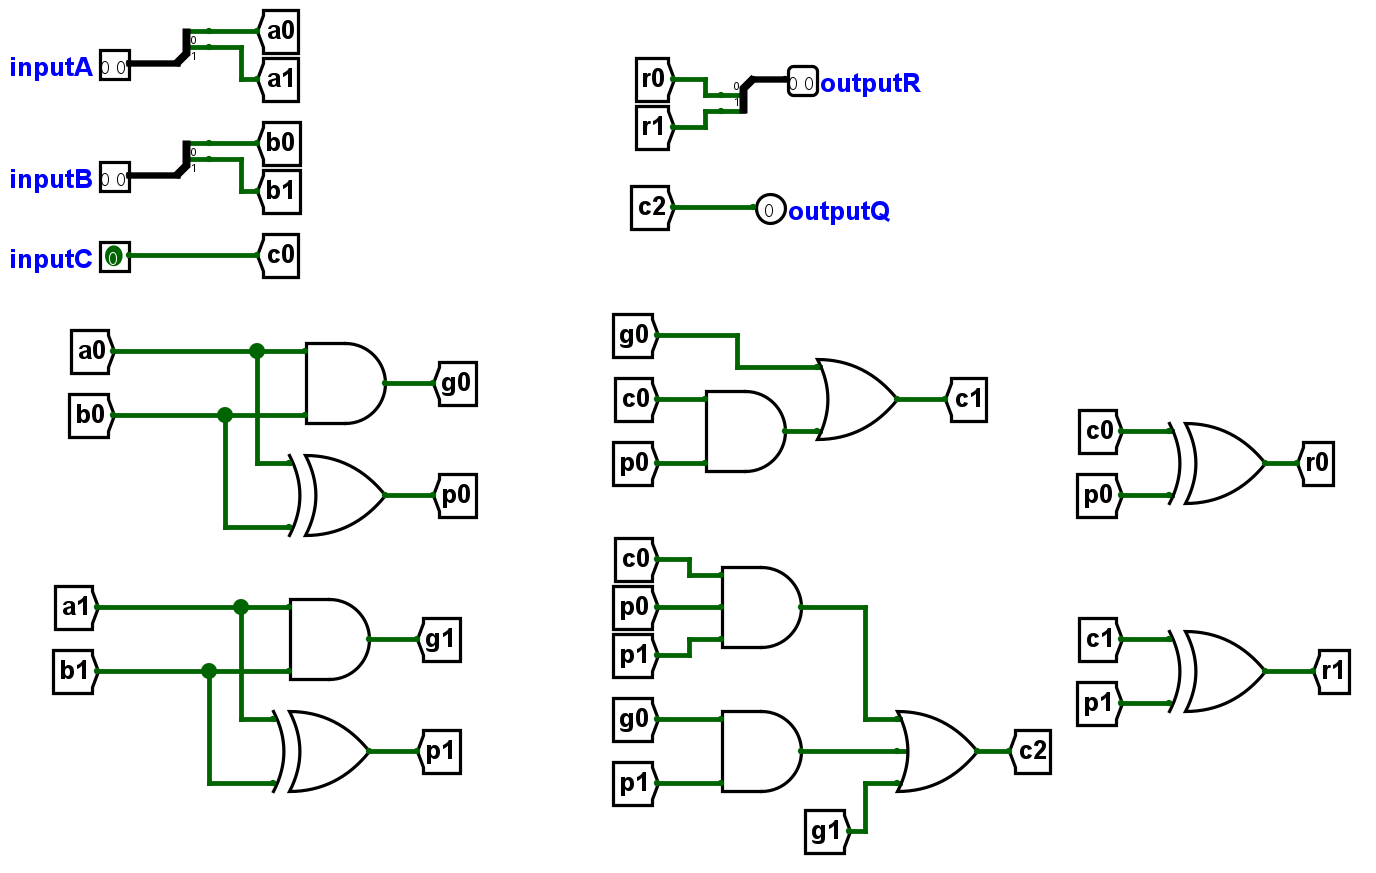
\includegraphics[width=0.8\textwidth]{circuit.png}
    \caption{A 2-bit arithmetic circuit}
    \label{fig:circuit}
\end{figure}

(a) Draw the truth table of this circuit.\textbf{[10 pt]}

(b) Which kind of arithmetic operation (addition, subtraction, multiplication, division, shift, or comparison) is performed by this circuit? What are the advantages and disadvantages of the circuit in Fig.~\ref{fig:circuit} compared to the corresponding arithmetic circuit mentioned in \href{https://toast-lab.sist.shanghaitech.edu.cn/courses/CS110@ShanghaiTech/Spring-2024/lecture_notes/L09.\%20Digital\%20circuits\%20and\%20systems\%201.pdf}{Digital circuits I}?\textbf{[10 pt]}

(c) Assume that all 2-input logic gates have 1 ns delay, all 3-input logic gates have 2 ns delay, and other delays are not considered. Calculate the max delay of this circuit.\textbf{[10 pt]}
\newpage
\begin{answer}[Question 1]
    (a)
    \begin{center}
        \begin{tabular}{ |c|c|c|c|c|c|c|c|c|c|c|c|c| }
            \hline
            $A_0$&$A_1$&$B_0$&$B_1$&$c_0$&$g_0$&$g_1$&$p_0$&$p_1$&$c_1$&$c_2$&$r_0$&$r_1$\\
            \hline
            0&0&0&0&0&0&0&0&0&0&0&0&0\\
            \hline
            0&0&0&0&1&0&0&0&0&0&0&1&0\\
            \hline
            0&0&0&1&0&0&0&0&1&0&0&0&1\\
            \hline
            0&0&0&1&1&0&0&0&1&0&0&1&1\\
            \hline
            0&0&1&0&0&0&0&1&0&0&0&1&0\\
            \hline
            0&0&1&0&1&0&0&1&0&1&0&0&1\\
            \hline
            0&0&1&1&0&0&0&1&1&0&0&1&1\\
            \hline
            0&0&1&1&1&0&0&1&1&1&1&0&0\\
            \hline
            0&1&0&0&0&0&0&0&1&0&0&0&1\\
            \hline
            0&1&0&0&1&0&0&0&1&0&0&1&1\\
            \hline
            0&1&0&1&0&0&1&0&0&0&1&0&0\\
            \hline
            0&1&0&1&1&0&1&0&0&0&1&1&0\\
            \hline
            0&1&1&0&0&0&0&1&1&0&0&1&1\\
            \hline
            0&1&1&0&1&0&0&1&1&1&1&0&0\\
            \hline
            0&1&1&1&0&0&1&1&0&0&1&1&0\\
            \hline
            0&1&1&1&1&0&1&1&0&1&1&0&1\\
            \hline
            1&0&0&0&0&0&0&1&0&0&0&1&0\\
            \hline
            1&0&0&0&1&0&0&1&0&1&0&0&1\\
            \hline
            1&0&0&1&0&0&0&1&1&0&0&1&1\\
            \hline
            1&0&0&1&1&0&0&1&1&1&1&0&0\\
            \hline
            1&0&1&0&0&1&0&0&0&1&0&0&1\\
            \hline
            1&0&1&0&1&1&0&0&0&1&0&1&1\\
            \hline
            1&0&1&1&0&1&0&0&1&1&1&0&0\\
            \hline
            1&0&1&1&1&1&0&0&1&1&1&1&0\\
            \hline
            1&1&0&0&0&0&0&1&1&0&0&1&1\\
            \hline
            1&1&0&0&1&0&0&1&1&1&1&0&0\\
            \hline
            1&1&0&1&0&0&1&1&0&0&1&1&0\\
            \hline
            1&1&0&1&1&0&1&1&0&1&1&0&1\\
            \hline
            1&1&1&0&0&1&0&0&1&1&1&0&0\\
            \hline
            1&1&1&0&1&1&0&0&1&1&1&1&0\\
            \hline
            1&1&1&1&0&1&1&0&0&1&1&0&1\\
            \hline
            1&1&1&1&1&1&1&0&0&1&1&1&1\\
            \hline
        \end{tabular}        
    \end{center}
    (b)
    it is a addition operation.


    Advantages: Shorter delay, capable of parallel computation across multiple bits;

    Disadvantages: Requires more logic gates.

    (c)

    the longest circuit path is c2$\rightarrow$3-or$\rightarrow$3-and$\rightarrow$p0/p1$\rightarrow$2-xor

    then the max delay is $2\times2+1\times1=5$
\end{answer}

\newpage
\section{SDS}
Draw a counter that counts from 0 to 5 using three D flip-flops (each flip-flops represents one output bit) and some 2-input logic gates (AND, OR, NOT). Please use the method taught in class to build a Moore FSM that implements the circular counter. Complete the state transition logic and output logic. \textbf{[35 pt]}
\begin{figure}[hp]
    \centering
    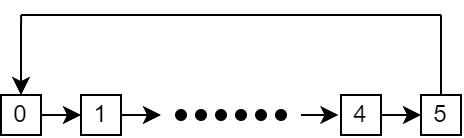
\includegraphics[height=2cm]{q2.png}
    \caption{The counter cycles through the process of counting from 0 to 5.}
    \label{fig:q2}
\end{figure}
\begin{answer}[Question 2]
    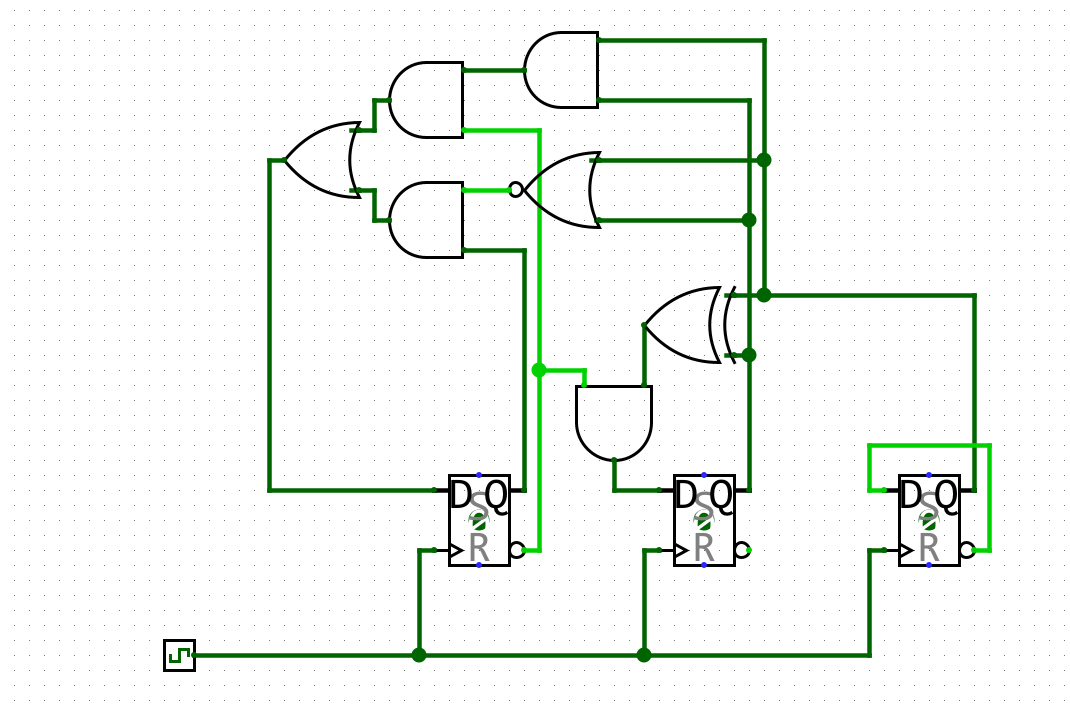
\includegraphics[height=6cm]{Screenshot from 2024-04-23 14-42-25.png}

    the FSM is:
    \begin{center}
        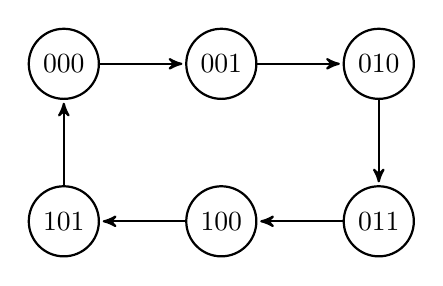
\begin{tikzpicture}[->,>=stealth',shorten >=1pt,auto,node distance=2cm,
        thick,base node/.style={circle,draw}, real node/.style={double,circle,draw}]
        \node[state] (1) {000};
        \node[state](2)[right of=1]{001};
        \node[state](3)[right of=2]{010};
        \node[state](4)[below of=3]{011};
        \node[state](5)[below of=2]{100};
        \node[state](6)[below of=1]{101};
        
        \path[]
        (1) edge node {} (2)
        (2) edge node {} (3)
        (3) edge node {} (4)
        (4) edge node {} (5)
        (5) edge node {} (6)
        (6) edge node {} (1);
    \end{tikzpicture}
    \end{center}

    \begin{center}
        \begin{tabular}{|c|c|c||c|c|c|}
            \hline
            $a_{2_{t-1}}$&$a_{1_{t-1}}$&$a_{0_{t-1}}$&$a_{2_t}$&$a_{1_t}$&$a_{0_t}$\\
            \hline
            0&0&0&0&0&1\\
            \hline
            0&0&1&0&1&0\\
            \hline
            0&1&0&0&1&1\\
            \hline
            0&1&1&1&0&0\\
            \hline
            1&0&0&1&0&1\\
            \hline
            1&0&1&0&0&0\\
            \hline
        \end{tabular}
    \end{center}

    $\Rightarrow$ after simplify, the output is: 
    $$a_0=\overline{a_0}$$
    $$a_1=(a_0\oplus a_1)\overline{a_2}$$
    $$a_2=a_0a_1\bar{a_2}+\overline{a_0+a_1}a_2$$
\end{answer}

\newpage
\section{Finite state machine}

The function of a vending machine which sells bottles of soda is described below:

\begin{itemize}
\item[$\bullet$] Each bottle costs \$1.50. 
\item[$\bullet$] The machine only accepts \$0.50 and \$1 coins. If a customer inserts enough coins, the machine will dispense a bottle of soda (FSM will output ``1", otherwise ``0'') and returns change if needed , e.g., the output of DISPENSE states may be ``1 \$0.5", other states' output may be ``0 \$0''.
\item[$\bullet$] The process happens one coin at a time, and there is no simultaneous insertion of multiple coins or shipping of multiple bottles. After each transaction, the vending machine enters the IDLE state.
\item[$\bullet$] We don’t need to account for a scenario where a customer inserts coins but decides not to make a purchase.
\end{itemize}


(a) Draw the FSM (Moore machine) for this vending machine.\textbf{[15 pt]}

(b) Draw the FSM (Mealy machine) for this vending machine.\textbf{[10 pt]}

(c) Could Moore machines and Mealy machines be converted into each other to implement the same function? Compare their difference.\textbf{[10 pt]}
\begin{answer}[Question 3]
    (a)

    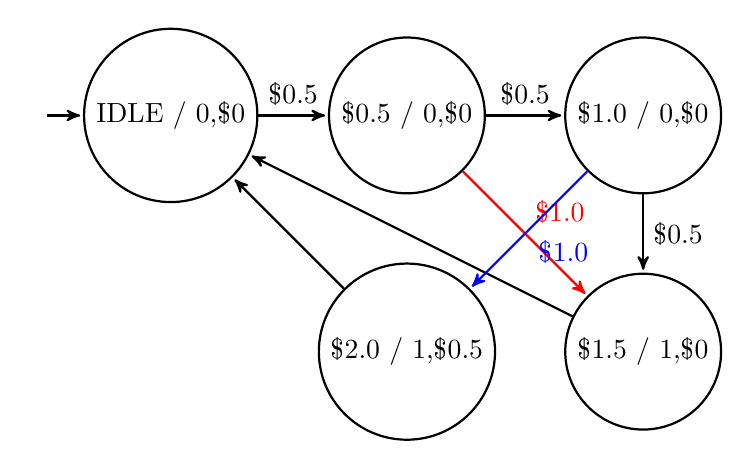
\begin{tikzpicture}[->,>=stealth',shorten >=1pt,auto,node distance=3cm,
        thick,base node/.style={circle,draw}, real node/.style={double,circle,draw}]
        \node[initial,state,initial text={}] (1) {IDLE / 0,\$0};
        \node[state](2)[right of=1]{\$0.5 / 0,\$0};
        \node[state](3)[right of=2]{\$1.0 / 0,\$0};
        \node[state](4)[below of=3]{\$1.5 / 1,\$0};
        \node[state](5)[below of=2]{\$2.0 / 1,\$0.5};
        
        \path[]
        (1) edge node {\$0.5} (2)
        (2) edge node {\$0.5} (3)
        (3) edge node {\$0.5} (4)
        (2) [red]edge [red]node {\$1.0} (4)
        (4) edge node {} (1)
        (3) [blue]edge [blue]node {\$1.0} (5)
        (5) [black]edge node {} (1);
    \end{tikzpicture}

    (b)

    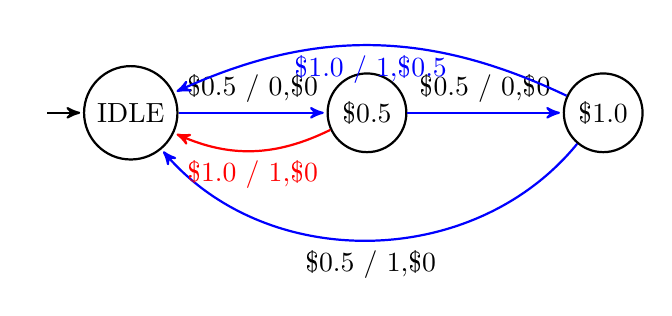
\begin{tikzpicture}[->,>=stealth',shorten >=1pt,auto,node distance=3cm,
        thick,base node/.style={circle,draw}, real node/.style={double,circle,draw}]
        \node[initial,state,initial text={}] (1) {IDLE};
        \node[state](2)[right of=1]{\$0.5};
        \node[state](3)[right of=2]{\$1.0};
        
        \path[]
        (1) edge node {\$0.5 / 0,\$0} (2)
        (2) edge node {\$0.5 / 0,\$0} (3)
        (3) [black, bend right=-50]edge node {\$0.5 / 1,\$0} (1)
        (2) [red, bend right=-25]edge [red]node {\$1.0 / 1,\$0} (1)
        (3) [blue, bend right=25]edge [blue]node {\$1.0 / 1,\$0.5} (1);
    \end{tikzpicture}

    (c)

    They can be converted into each other.

    The differences are: 1. Mealy Machines may have fewer nodes. 2. The outputs of a Mealy Machine depends on the current state and current input, while the outputs of a Moore Machine only depends the current state.
\end{answer}

\end{document}
